\section{Differential branching fraction}
 The values for the absolute branching fraction of the
 \decay{\Lb}{\Lz\mumu} decay, obtained by multiplying the relative
 branching fraction by the absolute branching fraction of the
 normalisation channel,
 $\BF(\decay{\Lb}{\jpsi\Lz})=(6.3\pm1.3)\times10^{-4}$~\cite{Agashe:2014kda},
 are given in Fig.~\ref{fig:mass_fit_smallbins} and summarised in
 Table~\ref{tab:AbsBR}, where the SM predictions are obtained from
 Ref.~\cite{Detmold:2012vy}.  The relative branching fractions are
 given in the Appendix.

 Evidence for signal is found in the \qsq region between the
 charmonium resonances and in the interval $0.1 < \qsq < 2.0$
 \gevgevcccc, where an increased yield is expected due to the
 proximity of the photon pole.  The uncertainty on the branching
 fraction is dominated by the precision of the branching fraction for
 the normalisation channel, while the uncertainty on the relative
 branching fraction is dominated by the size of the data sample
 available.  The data are consistent with the theoretical predictions
 in the high-\qsq region but lie below the predictions in the low-\qsq
 region.

\begin{table}[tbph]
\centering
\renewcommand{\arraystretch}{1.2}
\caption{Measured differential branching fraction of
  \decay{\Lb}{\Lz\mumu}, where the uncertainties are statistical, systematic and
 due to the uncertainty on the normalisation mode, \decay{\Lb}{\jpsi\Lz}, respectively.}
\begin{tabular}{ccccccc}
  \qsq interval  [\gevgevcccc] & &\multicolumn{5}{c}{$\deriv \BF(\decay{\Lb}{\Lz\mumu})/\deriv\qsq \cdot 10^{-7} [(\gevgevcccc)^{-1}]$} \\
\hline
0.1 -- 2.0    &    &0.36  &  $^{+\,0.12}_{-\,0.11}$   & $^{+\,0.02}_{-\,0.02}$ & $\pm\,0.07$ \\
2.0 -- 4.0    &    &0.11  &  $^{+\,0.12}_{-\,0.09}$   & $^{+\,0.01}_{-\,0.01}$ & $\pm\,0.02$ \\
4.0 -- 6.0    &    &0.02  &  $^{+\,0.09}_{-\,0.00}$   & $^{+\,0.01}_{-\,0.01}$ & $\pm\,0.01$ \\
6.0 -- 8.0    &    &0.25  &  $^{+\,0.12}_{-\,0.11}$   & $^{+\,0.01}_{-\,0.01}$ & $\pm\,0.05$ \\

11.0 -- 12.5  &    &0.75  &  $^{+\,0.15}_{-\,0.14}$   & $^{+\,0.03}_{-\,0.05}$ & $\pm\,0.15$ \\
15.0 -- 16.0  &    &1.12  &  $^{+\,0.19}_{-\,0.18}$   & $^{+\,0.05}_{-\,0.05}$ & $\pm\,0.23$ \\
16.0 -- 18.0  &    &1.22  &  $^{+\,0.14}_{-\,0.14}$   & $^{+\,0.03}_{-\,0.06}$ & $\pm\,0.25$ \\
18.0 -- 20.0  &    &1.24  &  $^{+\,0.14}_{-\,0.14}$   & $^{+\,0.06}_{-\,0.05}$ & $\pm\,0.26$ \\

\hline
1.1 -- 6.0    &    &0.09  &  $^{+\,0.06}_{-\,0.05}$   & $^{+\,0.01}_{-\,0.01}$ & $\pm\,0.02$ \\
15.0 -- 20.0  &    &1.20  &  $^{+\,0.09}_{-\,0.09}$   & $^{+\,0.02}_{-\,0.04}$ & $\pm\,0.25$ \\
 \end{tabular}
\label{tab:AbsBR}
\end{table}

 \begin{figure}[tbph]
 \centering
%% \includegraphics[width=0.8\textwidth]{images_and_tables/BR/combined_result_absolute_2err_rareErrIn.pdf}
 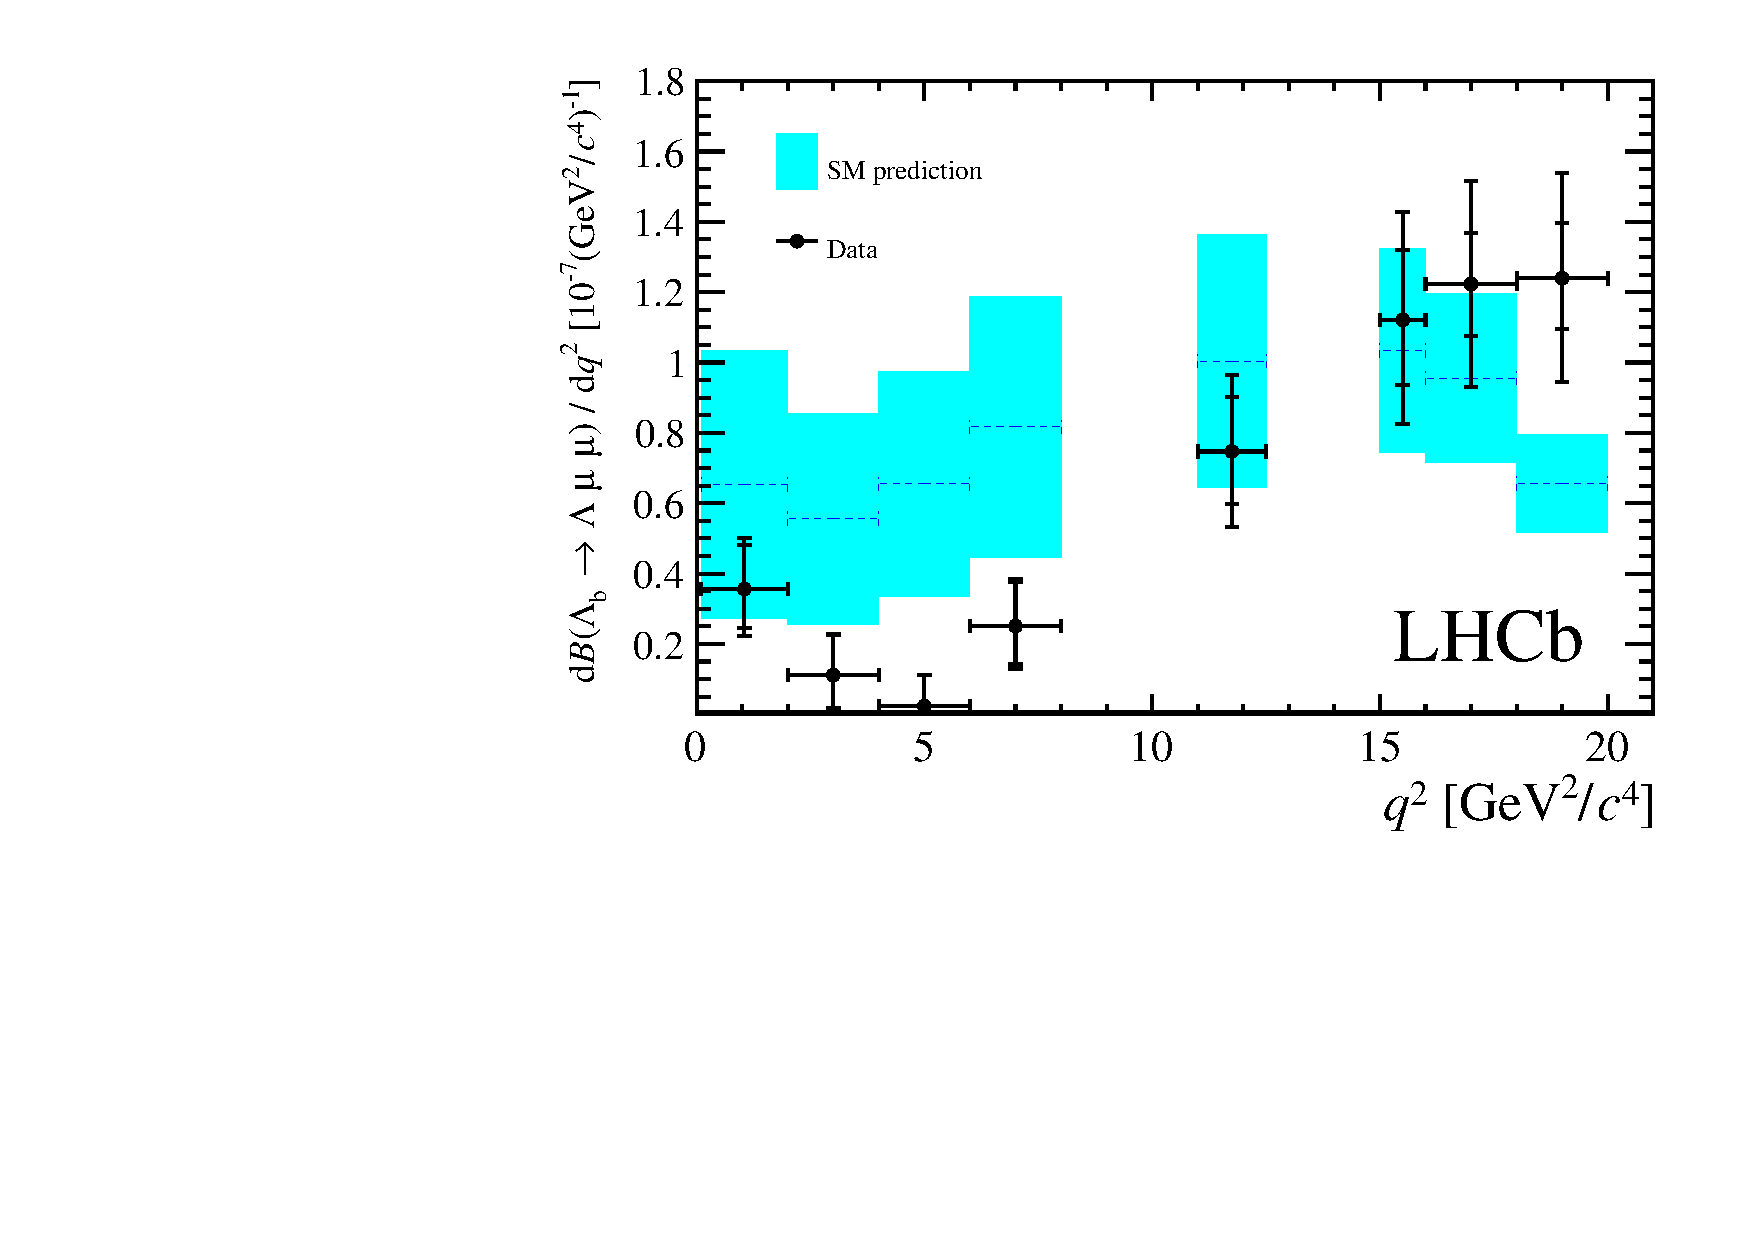
\includegraphics[width=0.8\textwidth]{figure5.pdf}
 \protect\caption{ Measured \protect\decay{\Lb}{\Lz\mumu} branching
   fraction as a function of \qsq with the predictions of the SM
   \cite{Detmold:2012vy} superimposed.  The inner error bars on data
   points represent the total uncertainty on the relative branching
   fraction (statistical and systematic); the outer error bar also
   includes the uncertainties from the branching fraction of the
   normalisation mode.}  \protect\label{fig:mass_fit_smallbins}
 \end{figure}

